\def\year{2017}\relax
%File: formatting-instruction.tex
\documentclass[letterpaper]{article}
\usepackage{aaai17}
\usepackage{times}
\usepackage{helvet}
\usepackage{courier}
\usepackage{url} 
\usepackage{multicol}
\usepackage{array}
\usepackage{xcolor}
\usepackage{subcaption}
\usepackage{graphicx}
\graphicspath{ {images/} }  
\frenchspacing
\setlength{\pdfpagewidth}{8.5in}
\setlength{\pdfpageheight}{11in}
\pdfinfo{
/Title (Nasty, Brutish, and Short: What Makes Election News Popular on Twitter?)
/Author (Sophie Chou, Deb Roy) 
/Keywords (Twitter, News, Virality)}
\setcounter{secnumdepth}{0}  
 \begin{document}
% The file aaai.sty is the style file for AAAI Press 
% proceedings, working notes, and technical reports.
%
\title{Nasty, Brutish, and Short:\\
What Makes Election News Popular on Twitter?}
\author{Sophie Chou\\
MIT Media Lab\\
Cambridge, MA, USA\\
soph@media.mit.edu\\
\And
Deb Roy\\
MIT Media Lab\\
Cambridge, MA, USA\\
dkroy@media.mit.edu\\
}
\maketitle
\begin{abstract}
During the 2016 U.S. presidential elections, Twitter served as an important platform for the spread of news articles, which have significant influence on public opinion. Yet the sharing of stories is often based on innate emotional triggers, seldom rational. In our research, we seek to examine whether the emotional vocabulary of political news stories can lead to their popularity.To explore these questions, we construct a corpus of 2,650 articles from 12 different news publications over 5 months, conncted with the 123,113 tweets by 20,964 Twitter users that share them. Using the Harvard Inquirer lexicons, we automatically code stories for emotionality and positivity. We then run regressions between the independent variables of story length, emotionality, and positivity and the dependent variable of number of shares across 7 different political divisions of Twitter users, as well as the collective dataset. On the whole, we find Twitter users to favor stories that are Hobbesian in nature: nasty (negative in positivity), brutish (high in emotionality), and short (low in word count). However, differences emerge when considering different levels of political engagement among users.
\end{abstract}

 
\section{Introduction}
In the changing landscape of both journalism and politics, social media is playing an increasingly large role in mobilizing and spreading information to citizens. A Pew Research survey from August 2015 showed that nearly two-thirds of adults in the U.S. who are on Twitter use the platform to get news \cite{pew-Twitter-news}. During an election year, the news on Twitter has the power to influence public opinion, which, in turn, impacts political outcomes.

But the popularity of sharing articles on social media also marks an important shift in the role of the news consumer from armchair reader to information propagator. Whereas news used to be broadcast to the reader, each reader now has the powerful potential to broadcast stories to his or her own audience. Yet previous work, including Berger and Milkman's study on what makes the New York Times' ``most emailed list'' and Hansen et. al.'s research on sentiment and news-sharing, show that the impulse to share content is often predictably emotional in nature \cite{berger2012makes,hansen2011good}. In short, the desire to share a certain story is often universally impulsive, regardless of context. In the case of political news, this impulse can have a large impact on reach of political messages -- an impact that is not always equally distributed. 

 \subsection{Hypotheses}
We ask the following question in our research: Does the emotional vocabulary of political news stories have an impact on its Twitter popularity that persists beyond political affiliation? To test this question, we focus on three key aspects of stories: length, emotionality, and positivity. We hypothesize:

\begin{itemize} 
    \item \textbf{H1:} Story length has a \emph{negative} correlation with Twitter shares, due to the effects of the internet attention economy and overexposure to political media \cite{goldhaber1997attention}.
    \item \textbf{H2:} Emotionality has a \emph{positive} correlation with Twitter shares, consistent for viral content in general \cite{berger2012makes}.
    \item \textbf{H3:} Positivity has a \emph{negative} correlation with Twitter shares, based on the classical news value that ``bad news is more newsworthy than good news'', and all the more so for political news \cite{galtung1965structure}. 

\end{itemize}

Prior literature has shown there to be a link between following a political candidate and underlying political orientation, so we group users by candidates followed to look for differences in sharing behavior \cite{colleoni2014echo}. For each of these three independent variables we repeat analyses across three views of the data: first, the entire dataset; then, by political candidate followed amongst users who follow only one candidate; and finally, by the number of political candidates followed (degree of political engagement). 
\section{Data Collection} 

\subsection{News Dataset}
For our news dataset, we scraped articles from the RSS feeds of 12 publications every hour from January 1, 2016 (the start of the election year) to May 1, 2016. This captures the bulk of primary election coverage.

We track the following outlets: CNN, Fox News, the New York Times, The Wall Street Journal, The Washington Post, The Los Angeles Times, The Associated Press, McClatchy, Politico, Buzzfeed, The Huffington Post, and NPR. These publications comprise a mix of ``legacy'' (over a hundred years old) and ``new'' media (founded online within the last 10 years) outlets, include stories directed towards different parts of the political spectrum (based on a 2014 survey from Pew), and include a variety of primary media formats (television, paper, online, radio) as well as specialties \cite{PoliticalPolarization}.   

Articles are processed in a 3-step pipeline. After collecting the links to the full content of the news stories from each publication's RSS feed, we pass each link to a structured content parser that extracts entities and features from the raw HTML. The story text is then passed into a binary MaxEnt classifier for election news. The classifier, which was built for prior research, performs with a F-score of 0.90 \cite{vijayaraghavan-thesis}. 

\subsection{Tweets Dataset}
We start with the firehose of all tweets between January 1, 2016 and May 1, 2016 in our data process. Tweets pass through a similiar pipeline as news stories. First, we sort all tweets with an election classifier, built for prior research, which has been shown to be able to detect election-related tweets with an F-score of 92\% \cite{vvr_electome2016}. We then filter by those that share a link (which might potentially be a news story). We collect and sort a total of 16,667,685 tweets as election-related and containing at least one URL in the text, an average of 4,000,000 per month and 140,000 per day.

\subsection{Combined Dataset}
To connect articles with tweets, we expand all links in tweets from ``t.co'' format (16.6 million), then use regular expressions to see if the final destination of the expanded link matches a query-truncated URL of a story in our database. In total, we found that 30\% of the election stories we tracked were shared on Twitter during the time period of January 1st through May 1st. There were 137,986 tweets that contained a link to 6,911 unique stories (out of 22,960). We eliminated any stories that were shared by less than 10 tweets to remove obscure articles. This left a total of 2,650 distinct articles shared in 123,113 tweets by 20,956 Twitter users.

\subsubsection{Descriptive Findings}
Story sharing behavior follows an approximate power law distribution. On average, stories are shared 46 times. CNN, Politico, and Fox have the highest number of stories shared by tweets in our dataset (fig. \ref{fig:story-stats}-A). This is likely due to the volume of and focus on political content for these outlets. Coding each story by the candidate's name that appears the most, Trump has nearly three times as many featured stories compared to runner-ups Ted Cruz and Hillary Clinton (see fig. \ref{fig:story-stats}-B). High coverage of Cruz in stories is likely due to his association to Trump as a Republican runner-up: 96\% of stories where Cruz is the most-mentioned candidate feature Trump as the second-most frequently occuring.
%Donald Trump is by far the most ``tweetable'' candidate, dominating the top 10 most-shared list with 7 out of 10 stories featuring his name in the title. 

\begin{figure}[t!]
\centering 
  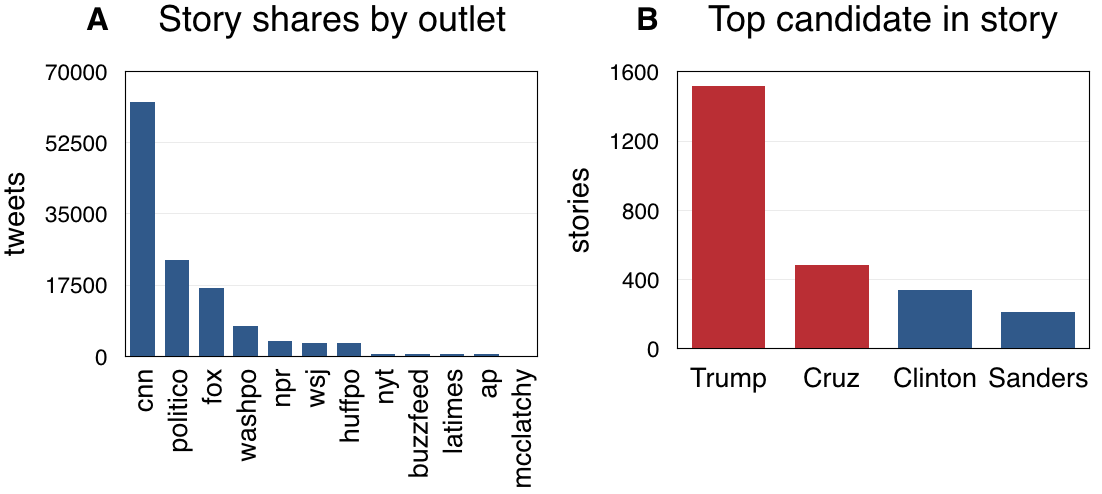
\includegraphics[width=\linewidth]{story-stats}   
    \caption{Popularity of stories, candidates in stories
    \label{fig:story-stats}}
\end{figure}  

\section{Political and Emotional Metrics}
\subsection{Emotional Coding}
For the emotional coding of news articles, we use dictionaries from the Harvard General Inquirer, a lexicon that is popular for computerized content analysis \cite{stone1963computer}. In Berger and Milkman's study of online virality, automated coding using the LIWC system showed results that were significantly positively correlated with the output of manual coding \cite{berger2012makes}. The Inquirer is a public-use alternative to the LIWC system. In particular, we look at the \emph{Positiv} and \emph{Negativ} collections, a set of 1,915 well-established words signifying positive outlook and 2,291 words signifying negative outlook. Repeating the same metrics from Berger and Milkman's study, we calculate emotionality as $\frac{count(positiv \mid negativ)}{count(words)}$ and positivity as $\frac{count(positiv)}{count(words)} - \frac{count(negativ)}{count(words)}$.

\subsection{Political Engagement}  
For general levels of political engagement, we look at the number of political candidates a Twitter user follows as a proxy for how likely they are to share political news. 36\% of Twitter users in our dataset follow none of the four political candidates, followed by 31\% who follow one candidate, 20\% who follow two, and 13\% who follow three or more candidates (fig. \ref{fig:levels-of-engagement-charts}-A). We see a negative curvlinear relationship between the number of candidates followed (level of observed political engagement) and the ratio of political news tweets per user, which may suggest lower volume but higher deliberation in users more engaged (see fig. \ref{fig:levels-of-engagement-charts}-B).

For our analyses, we segment levels of political engagement into three categories: \textbf{the unaffiliated} (those who follow no presidential candidates, but do tweet about political news), \textbf{the loyal} (those who follow one and only one presidential candidate, and tweet about political news), and \textbf{the political aficionados} (those who follow all 4 (or more) candidates, and tweet about political news).  

\subsubsection{Candidate Followership}
Our dataset contains 6,406 unique single-candidate Twitter users. At the time of data collection completion (May 1, 2016), the top two candidates by delegate count in each party were Hillary Clinton (D), Bernie Sanders (D) and Donald Trump (R) and Ted Cruz (R), so we split users into these four groups. Trump-only followers lead with about 31\% of all single-candidate users, followed closely by Clinton-only (29\%), then Sanders (25\%) and Cruz (14\%). 37\% of tweets sharing articles come from Trump-only followers versus 27\% for Clinton-only, 20\% for Sanders-only, and 14.6\% for Cruz. Again, across all four segments, Republican candidate Trump leads the top number of mentions in stories shared (see fig. \ref{fig:who-shares-what}).
 
\begin{figure}[t!]  
\centering 
  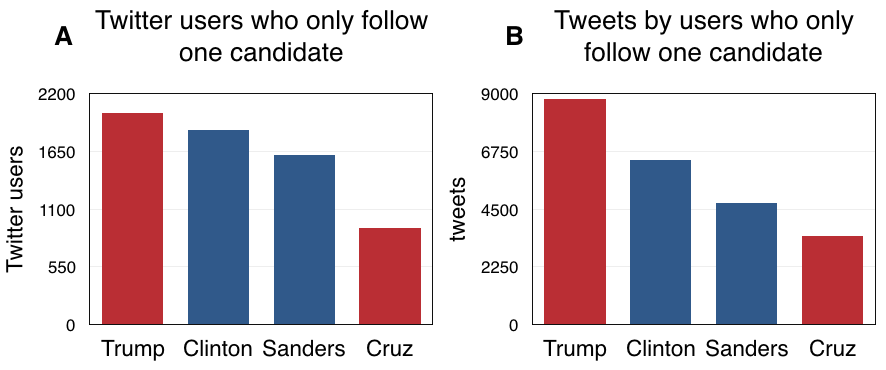
\includegraphics[width=\columnwidth]{single-candid-charts}  
   \caption{Single candidate followers
     \label{fig:single-candid-charts}}
\end{figure} 

\begin{figure}[t!] 
\centering 
 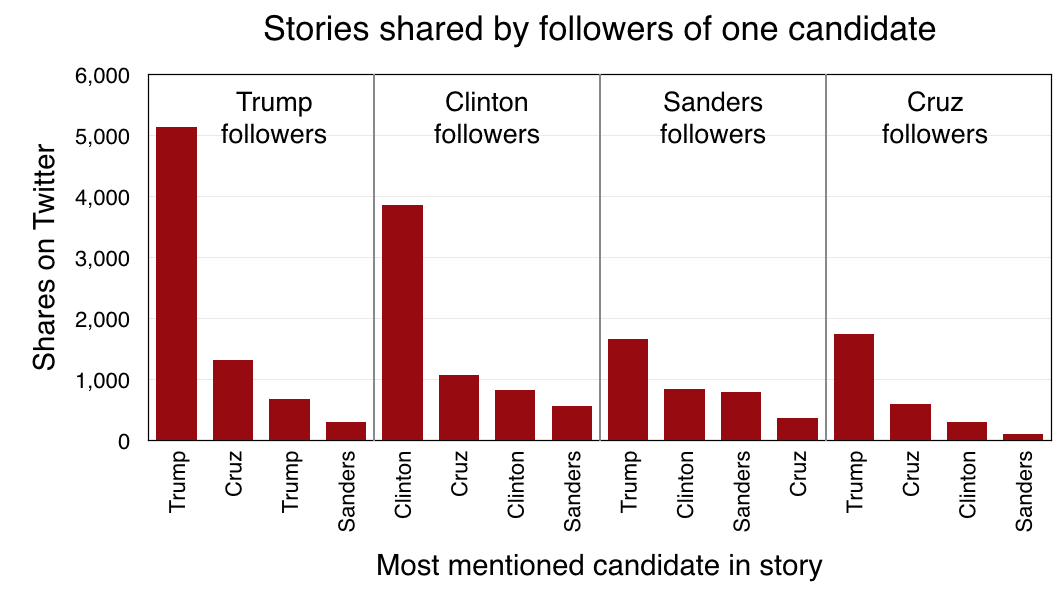
\includegraphics[width=1.0\columnwidth]{who-shares-what}  
  \caption{Stories shared by followers of one candidate 
    \label{fig:who-shares-what}}
\end{figure}

\begin{figure}[t!] 
\centering  
  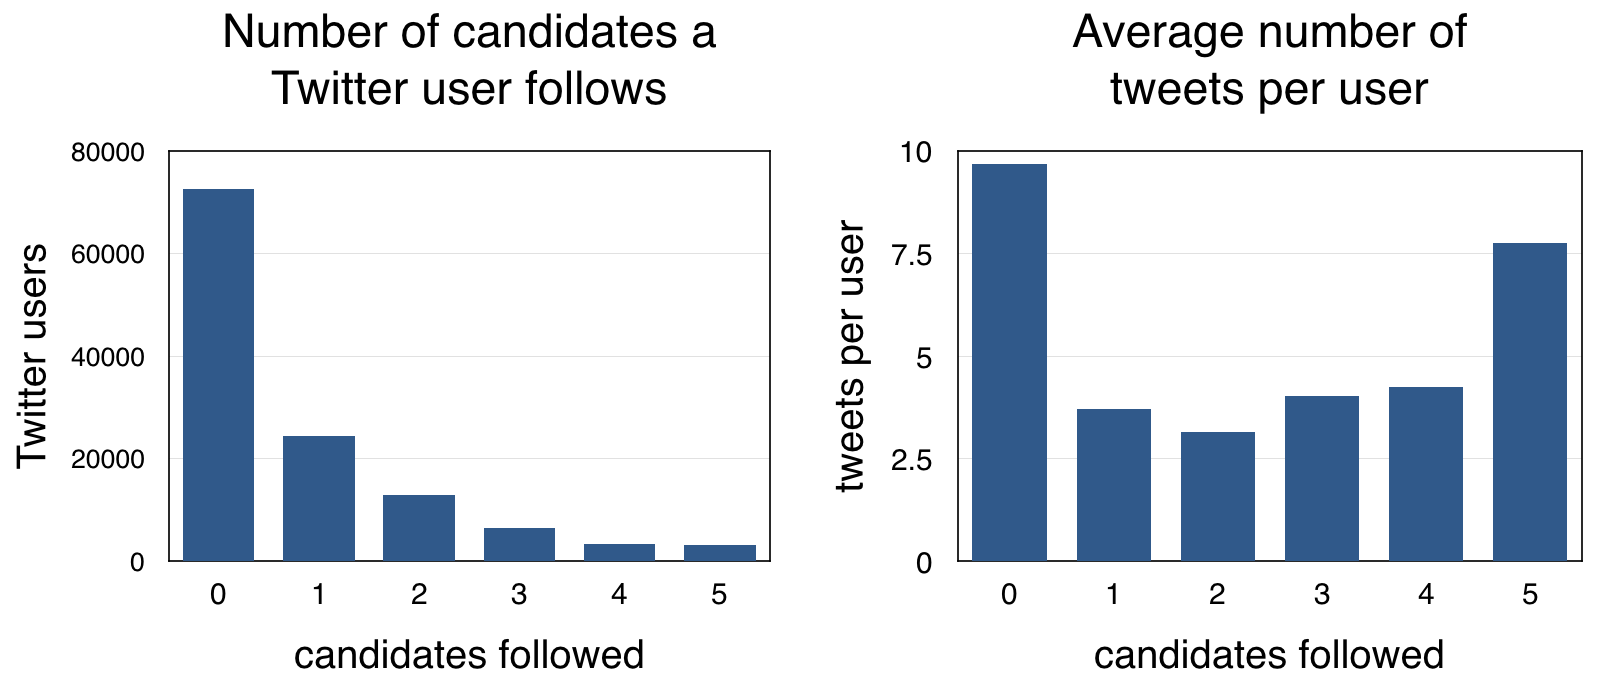
\includegraphics[width=\columnwidth]{levels-of-engagement-charts}  
  \caption{Behavior by candidates followed
    \label{fig:levels-of-engagement-charts}}
\end{figure} 

\section{Analysis}  
\subsection{Methodology}
Since our dependent variable, tweet volume, is a set of discrete counts that is positively truncated but overdispersed ($\theta > 1$), we use negative binomial regression models for our analysis \cite{scott1997regression}. We apply a log transformation on the independent variable of story length, as its distribution follows an approximate power law. Both emotionality and positivity are approximately normally distributed. In each case, we compare our findings to those using linear and Poisson regression models, and are able to achieve the same significant results. 
 
\subsection{All Data}
% Table created by stargazer v.5.2 by Marek Hlavac, Harvard University. E-mail: hlavac at fas.harvard.edu
% Date and time: Thu, Dec 22, 2016 - 11:14:33
\begin{table}[!htbp] \centering 
  \caption{Story Popularity vs. Story Traits, All Tweets} 
  \label{} 
\begin{tabular}{@{\extracolsep{5pt}}lc} 
\\[-1.8ex]\hline 
\hline \\[-1.8ex] 
 & \multicolumn{1}{c}{\textit{Dependent variable:}} \\ 
\cline{2-2} 
\\[-1.8ex] & num\_tweets \\ 
\hline \\[-1.8ex] 
 log(story length) & $-$0.088$^{***}$ \\ 
  & (0.017) \\ 
  & \\ 
 emotionality & 6.279$^{***}$ \\ 
  & (1.770) \\ 
  & \\ 
 positivity & $-$5.978$^{***}$ \\ 
  & (2.013) \\ 
  & \\ 
 constant & 4.296$^{***}$ \\ 
  & (0.117) \\ 
  & \\ 
\hline \\[-1.8ex] 
Observations & 2,650 \\ 
Log Likelihood & $-$12,761.660 \\ 
$\theta$ & 1.361$^{***}$  (0.035) \\ 
Akaike Inf. Crit. & 25,531.320 \\ 
\hline 
\hline \\[-1.8ex] 
\textit{Note:}  & \multicolumn{1}{r}{$^{*}$p$<$0.1; $^{**}$p$<$0.05; $^{***}$p$<$0.01} \\ 
\end{tabular} 
\end{table} 

Overall, we find a consistently negative correlation of high significance between story length and Twitter volume ($\beta=-0.088$, $p<0.01$). This aligns with our hypothesis that shorter stories are more likely to be shared, due to competing resources in the attention economy (\textbf{H1}). We find a consistently positive correlation of high significance between emotionality and Twitter volume ($\beta=6.279$, $p<0.01$), which confirms our second hypothesis and is aligned with viral content in general (\textbf{H2}). Finally, we find a consistently negative correlation of high significance between positivity and Twitter volume ($\beta=−5.978$, $p<0.01$). This supports our hypothesis that positivity has a \emph{negative} correlation with Twitter shares, due to the nature of political news and contrary to generalized findings from Berger and Milkman's study (\textbf{H3}).

\subsection{By Degree of Political Engagement}
For the three levels of political engagement (the unaffiliated, single-candidate followers, and political aficionados) we repeat the same methods and variables in determining our correlations. Again, we test all three models (OLS, Poisson, and NB) for consistency and report the results of the negative binomial model. Overall, we find that: 

The unaffiliated show the same patterns as the general dataset with a negative correlation between story length and Twitter shares ($\beta=-0.283$, $p<0.01$), positive correlation between emotionality and Twitter shares ($\beta=10.718$, $p<0.01$), and a negative correlation between positivity and Twitter shares ($\beta=-4.968$, $p<0.05$).

The loyal, on the other hand, show a slight positive correlation between story length and number of Twitter shares ($\beta=0.156$, $p<0.01$). For emotionality ($\beta=5.577$, $p<0.01$) and positivity ($\beta=-7.754$, $p<0.01$), the trends remain the same. We hypothesize that if following a single candidate can serve as a proxy for candidate loyalty, then perhaps the correlation signifies a willingness to read and share more complex content on behalf of the candidate and a deeper degree of political involvement.

We see the same effects for the political aficionado group, again, a small but significant positive correlation between story length and number of tweets ($\beta=0.205$, $p<0.01$). For this group, we found no significant correlations between emotionality and Twitter popularity, although there was a significant negative correlation (as before) between positivity and tweets ($\beta=-6.043$, $p<0.05$). Again, this suggests a potential difference in levels of engagement with political news. 

\subsection{By Candidate} 
We divide Twitter users into four segments: Trump-only, Clinton-only, Sanders-only, and Cruz-only followers and repeat the same regressions within each population. 

Overall, we were unable to find a significant difference in the direction of correlations in any of the three independent variables between these candidate groups and single-candidate followers (the loyal) at large. However, we did find differences in magnitudes of the coefficients; most notably a strong negative correlation between postivity and number of tweets for Trump-only followers, about two and a half times in magnitude ($\beta=-14.684$, $p<0.01$) of the rest of tweeters ($\beta=−5.978$, $p<0.01$). 

As discussed in the section above, all single-candidate followers that showed a significant correlation between story length and number of Twitter shares showed a slight positive correlation.

\section{Conclusion}
For the general population of election tweeters, we find that the stories that are more likely to be shared are shorter (\textbf{H1}), high in emotional words (\textbf{H2}), and less positive in tone (\textbf{H3}).

These results are aligned with our expectations of the limitations of the attention economy, the emotional nature of content virality, and the idea that ``bad news is more newsworthy than good news'', confirming Galtung and Ruge's classical theory, along with Hansen et. al.'s more recent work \cite{galtung1965structure,hansen2011good}.

However, there are small but significant differences in the number of political candidates a user followed and the length of the stories that were likely to be shared. Although the unaffiliated (and the general population of tweeters) tend to prefer short stories, both the loyal and political aficionados prefer longer stories. This suggests a deeper level of engagement with political content versus the general population, which might have a more impulsive mechanism for sharing articles, leaving room for future research.

\section{Limitations and Future Work}  
The 2016 elections were an unusual time period for both traditional and social media. Twitter users on all sides of the political spectrum focused on Donald Trump, which may have limited findings. Futhermore, our dataset was limited to a small but diverse set of publications. Potential ways to create a more complete dataset include: Expanding the set of publications tracked, using machine learning methods to match tweets with stories, applying a more nuanced analysis of the story text, and including additional signals in the Twitter user data, such as the inferred political leaning of the person and the interaction between that leaning and the content shared. Still, our analysis provides a first view of article sharing on Twitter in a unique and eventful election year with large responses on social media.

\bibliography{nasty-brutish-short-poster}
\bibliographystyle{aaai} 
 
\end{document}
